\section{Dataset Description}

The field campaign was conducted in a freshwater environment in the Amazon region (Itacoatiara, AM, Brazil), with georeferenced sampling points distributed to capture local spatial gradients. The dataset includes position in UTM 21S and physicochemical variables used as model inputs and outputs, and is publicly available in Mendeley Data \cite{assuncao2026dataset}. The spatial coverage of the campaign is shown in Fig.~\ref{fig:dataset_map}, and summary statistics of the prediction targets are reported in Table~\ref{tab:dataset_stats}.

Data collection followed a spatially distributed design to represent different lake micro-zones instead of repeatedly sampling a single coordinate, supporting spatial interpretation and local decision support (interpolation maps and composite screening indices). Measurements were consolidated into a tabular structure suitable for edge-oriented inference and reproducible training.

\subsection{Variables and Acquisition}
Input features were $x$, $y$, temperature (TEMP), apparent color in amber scale (COR\_A), and visual color index (COR\_V). Target variables were pH, dissolved oxygen (OD), and turbidity (TURB). The original field dataset comprises 60 georeferenced samples. The sampling design prioritized spatial representativeness over dense temporal repetition, consistent with the objective of generating interpretable spatial surfaces.

Table~\ref{tab:corr_analysis} reports the Pearson correlation between each input feature and each target in the original 60-sample dataset. Spatial coordinates and color indices are strongly associated with pH ($r=-0.85$ for $y$; $r=-0.79$ for COR\_A) and turbidity ($r=0.69$ and $r=0.68$, respectively), indicating exploitable spatial and optical gradients. In contrast, OD is weakly correlated with all available inputs ($|r| \leq 0.24$), which anticipates the higher difficulty of predicting this target in terms of explained variance with the current feature set.

\begin{table}[t]
\caption{Pearson correlation between input features and targets (original dataset, $n=60$).}
\label{tab:corr_analysis}
\centering
\footnotesize
\setlength{\tabcolsep}{6pt}
\begin{tabular}{lccc}
\toprule
Feature & pH & OD & TURB \\
\midrule
$x$ & $0.75$ & $-0.23$ & $-0.67$ \\
$y$ & $-0.85$ & $0.18$ & $0.69$ \\
TEMP & $-0.56$ & $0.24$ & $0.33$ \\
COR\_A & $-0.79$ & $0.05$ & $0.68$ \\
COR\_V & $-0.46$ & $0.08$ & $0.50$ \\
\bottomrule
\end{tabular}
\end{table}

\begin{figure}[t]
\centering
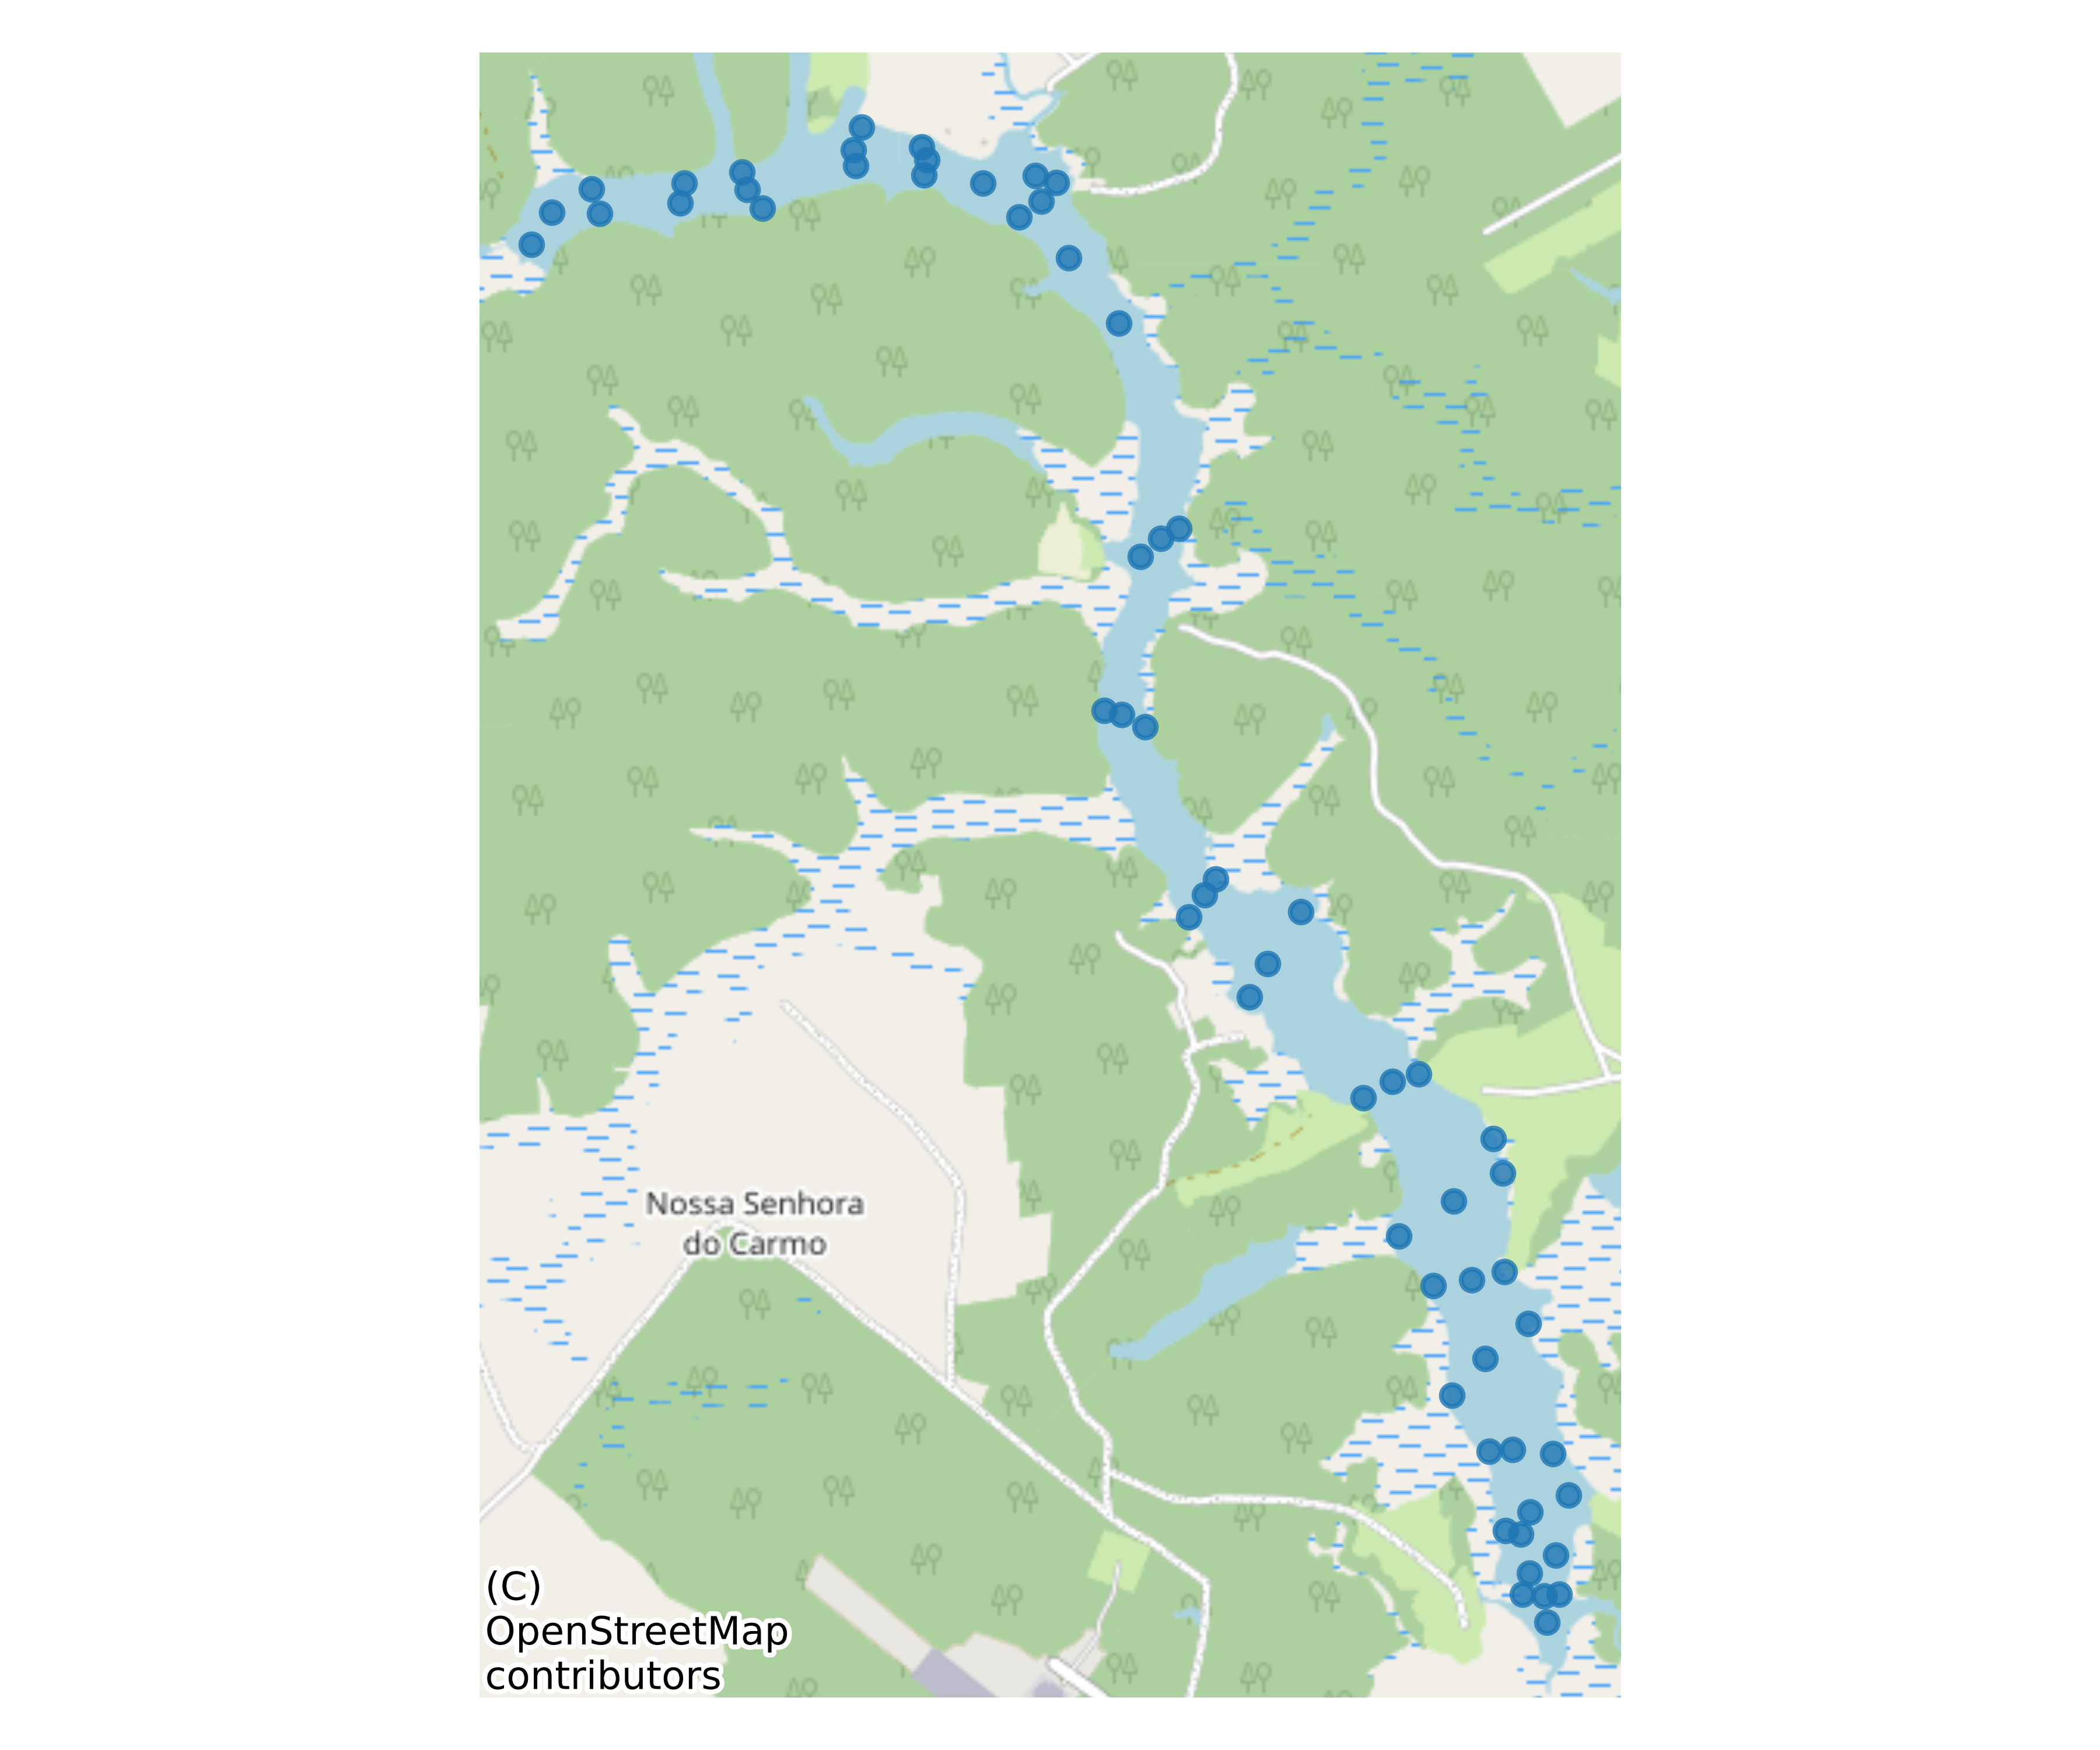
\includegraphics[width=0.64\linewidth]{map_points_osm_21S.png}
\caption{Sampling locations over OpenStreetMap basemap (UTM 21S).}
\label{fig:dataset_map}
\end{figure}

\begin{table}[t]
\caption{Target summary statistics in the original field dataset.}
\label{tab:dataset_stats}
\centering
\begin{tabular}{lcccc}
\toprule
Variable & Mean & Std & Min & Max \\
\midrule
pH & 5.73 & 0.31 & 5.15 & 6.50 \\
OD (mg/L) & 1.86 & 0.32 & 1.26 & 2.52 \\
Turbidity (NTU) & 2.77 & 1.37 & 0.06 & 6.18 \\
\bottomrule
\end{tabular}
\end{table}

\subsection{Data Augmentation}
Because the original dataset is small ($n=60$), synthetic augmentation was applied with factor $\times 10$ using light Gaussian perturbation ($\sigma=0.01$) in normalized space, yielding 600 training-support samples. This strategy was used to stabilize training and reduce split sensitivity, while preserving marginal distributions and physical plausibility. The augmented set is used for training support only and does not represent additional field measurements. Gaussian perturbation was adopted for its transparency and low distortion risk in this regime; alternative augmentation strategies for small tabular datasets, such as SMOTE-style interpolation for regression, mixup, and generative approaches (e.g., copula- or GAN-based synthesis), are natural candidates for a systematic comparison in future work.

To minimize distortion risk, augmentation was constrained to low-amplitude perturbations and evaluated with distributional checks and ablation analysis: the goal was to increase local density around observed samples and improve optimization stability across randomized splits, not to create synthetic dynamics absent from the field campaign.

Finally, the dataset should be interpreted as an initial regional benchmark rather than a universal hydrological representation. The current sampling supports comparative modeling and deployment analysis, while broader external generalization requires multi-season campaigns and additional freshwater sites with different hydrodynamic and anthropogenic profiles. The small sample size imposes concrete methodological limits: absolute metric values carry wide uncertainty, small differences between models may not be stable across resamplings, and single-season sampling cannot capture hydrological seasonality. These limits motivated the conservative protocol adopted here (repeated seeds, confidence intervals, and nonparametric tests) and bound the scope of the conclusions to comparative and deployment-oriented claims.
